\section{Carleman weights}

Carleman estimates introduce exponential weights that convert local decay into global constraints.

A typical transformation has the form
\[
v(x,t) = e^{\phi(x,t)} u(x,t),
\]
where \(\phi\) is a suitable weight function.

These estimates yield bounds of the form
\[
\| e^{\phi} u \| \le C \| e^{\phi} (i\partial_t + \Delta - V) u \|.
\]

Conceptually, this step changes the scale of the problem: the same mathematical object is viewed under a weighted norm.

\medskip

\noindent
\textbf{Interpretation.}
Smallness must act under the constraints imposed by the equation.

\begin{figure}[h]
\centering
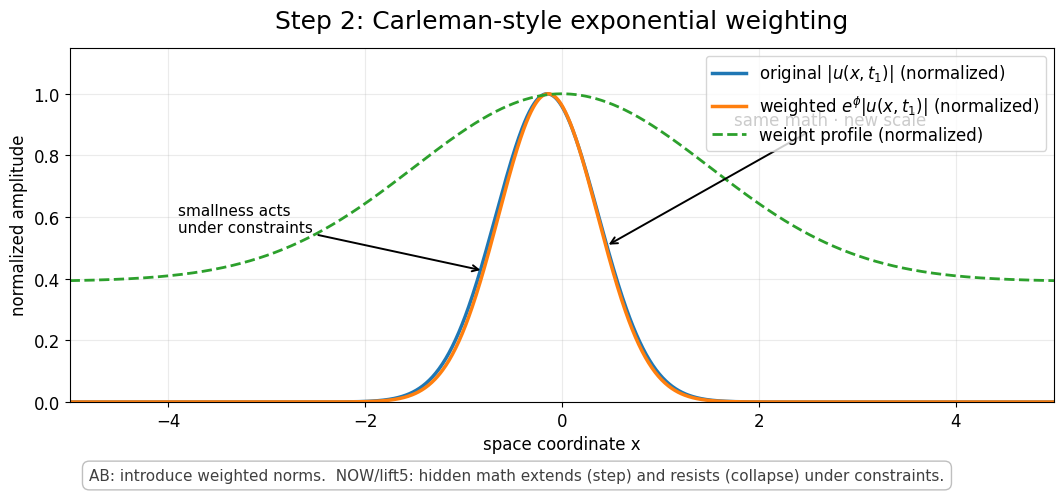
\includegraphics[width=\linewidth]{figures/step2_exponential_weight_code.png}
\caption{
Step 2. Exponential (Carleman) weighting: same math, new scale.
The weighted profile makes two-time smallness act under the constraints.
}
\end{figure}
